\chapter{Input Optics for high laser power}%

\section{Introduction}%
The Input Optics (IO)\footnote{The Input Optics was originally called the Input-Output Optics (IOO).} is one of many subsystems of the LIGO interferometers.  Its purpose is to deliver an aligned, spatially pure, mode-matched beam with phase-modulation sidebands to the power-recycled Fabry-Perot Michelson interferometer. The IO must prevent the backscattering of light into the laser, recover the beam reflected from the interferometer for signal detection and have high optical efficiency. It should not be a limiting noise source for DARM. 

There are four major components to the Input Optics subsystem:
\begin{itemize}
\item electro-optic modulator (EOM) \vspace{-10pt}%
\item mode cleaner cavity (MC) \vspace{-10pt}%
\item Faraday isolator (FI) \vspace{-10pt}%
\item mode matching telescope (MMT)
\end{itemize}
A layout is shown in Fig. \ref{fig:IOschematic} and the conceptual design is found in Ref. \cite{Camp1996InputOutput}. The focus of the U. of Florida's responsibility for the Input Optics is their design, fabrication, and performance under high laser powers. I elaborate on those aspects of the IO in this chapter, leaving the IO noise performance to a future discussion. 

\begin{figure}
\begin{centering}
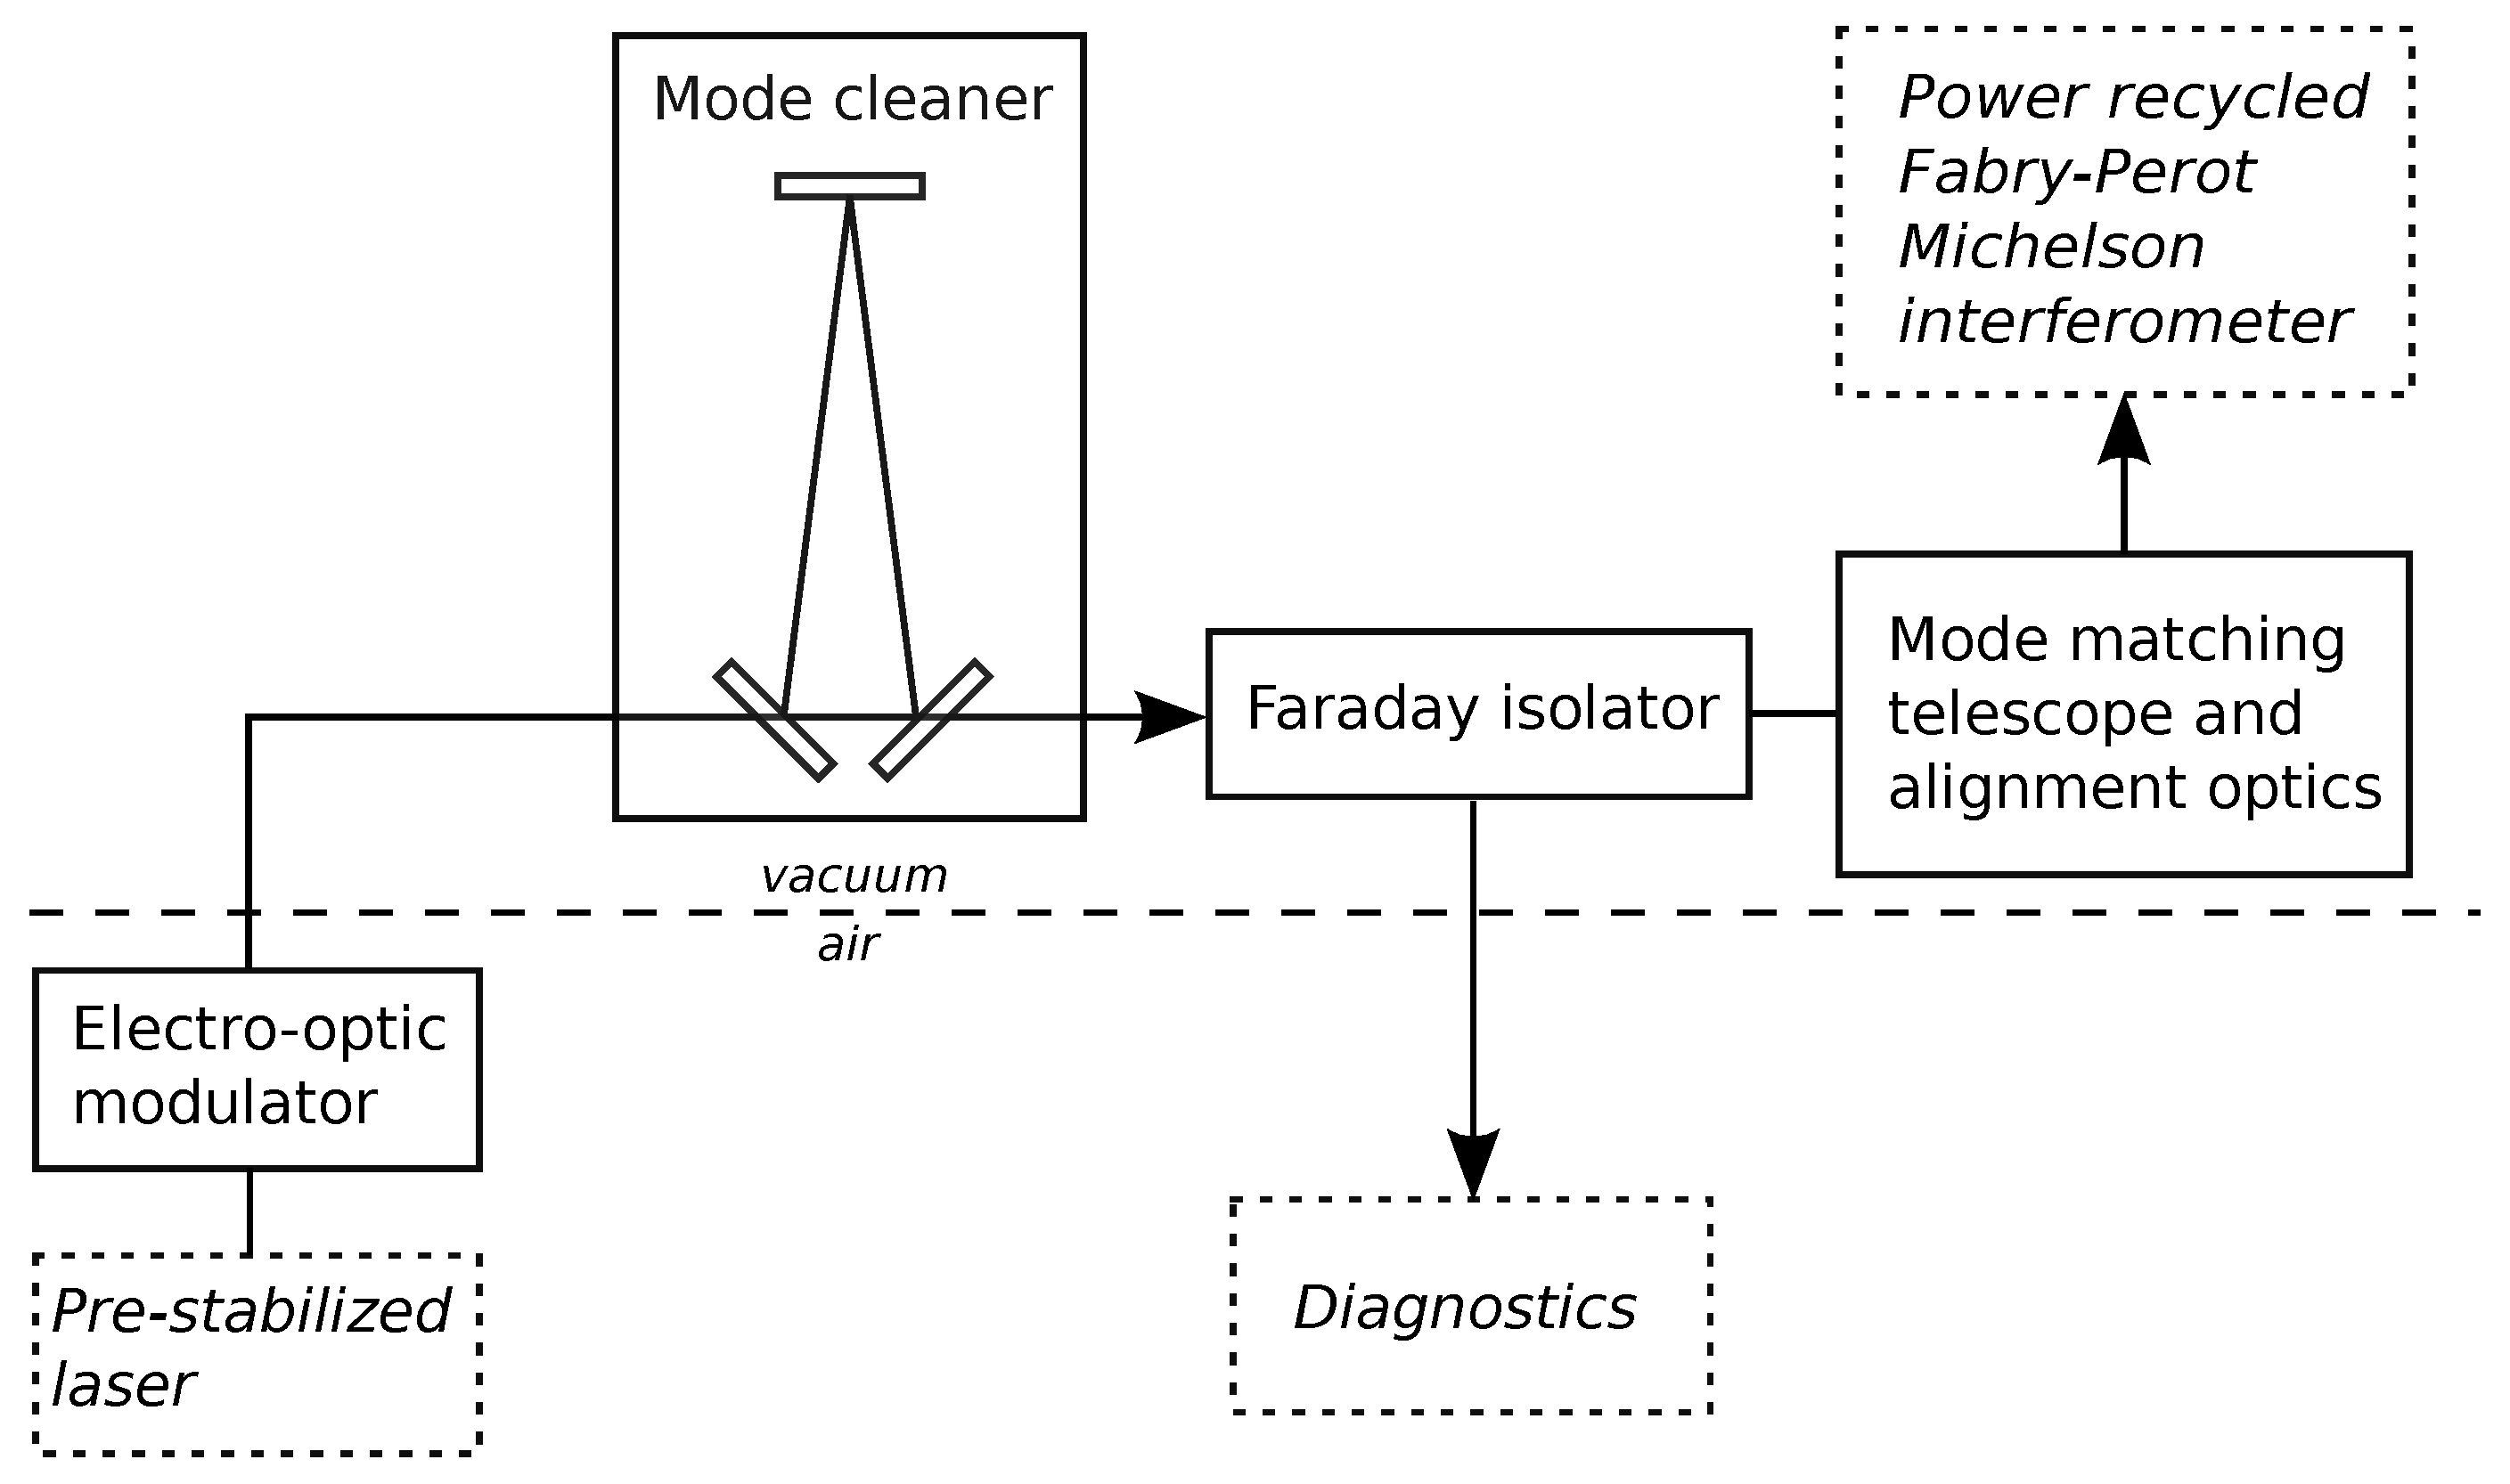
\includegraphics[width=0.8\textwidth]{/Users/kate/Documents/iopaper/figures/IOschematic.pdf}
\caption{Input Optics subsystem schematic. IO components are
  identified by solid rectangles. \textcolor{blue}{Make very detailed!
    OptoCad drawing, perhaps?}}
\label{fig:IOschematic}
\end{centering}
\end{figure}

\subsection{Problems in Initial LIGO}
The Initial LIGO interferometers were equipped with a 10~W laser, yet
operated with only 7~W input power due to radiation pressure induced
opto-mechanical instabilities in the arm cavities. The EOM sat
before the power control in the 10~W beam and the other components saw
anywhere up to 7~W laser power. The 7~W operational limit was not due
to the failure of the Input Optics; however, the quality of the IO
performance did degrade with power.

The single greatest fault of the Initial LIGO Input Optics was thermal drift in the Faraday isolator. The FI elements produced thermal deflection of the beam, leading to a significant beam drift between the interferometer's locked and unlocked states. The reflected beam, for instance, would wander completely off of a 0.5~cm diameter sensing photodiode during the course of powering up the interferometer. Measurements estimate there was a deflection of 1~mrad at the FI. This was mitigated at the time by the design, installation, and use of the REFL beam servo (RBS), an active beam steering system on the beam rejected by the isolator.

There were also known limits to the power the IO could sustain. For
example, thermal lensing in the Faraday isolator optics would start to
significantly alter the beam mode at powers greater than
10~W. Additionally, the absorptive FI elements would create thermal
birefringence with more power, degrading the optical efficiency and
isolation. Also, the Initial LIGO electro-optic modulators had an
operational power limit of around 10~W; anisotropic thermal lensing
made the EOMs unsuitable for much higher power. Finally, the mode
cleaner optics exhibited rather high absorption--enough such that
thermal lensing of the MC optics at higher powers would degrade the
mode quality of the beam and therefore its finesse. A power-dependent
mode mismatch into the interferometer would also be expected.

In addition to the thermal limitations of the Initial LIGO IO, optical
efficiency in delivering light from the laser into the interferometer
was not optimal during Initial LIGO. Of the light entering the Input
Optics chain, only 60\% remained by the time it reached the power
recycling mirror. In addition, only 83\% of the light reaching the
interferometer was coupled into the arm cavity mode at Livingston,
leaving room for improvement in the MMT design.



\section{Design of Enhanced LIGO Input Optics}

\subsection{Electro-optic modulator} 
The electro-optic modulator phase modulates carrier light to produce
RF sidebands that are needed for sensing the interferometer lengths
and angles \cite{Fritschel2001Readout}. Carrier light with field $E_0
e^{i \omega t}$ has first order sidebands with amplitude $E_0
J_1(\Gamma_i) e^{i (\omega + \Omega_i) t} + E_0 J_{-1}(\Gamma_i) e^{i
  (\omega - \Omega_i) t}$ addet to it, along with infinitely many
higher order sidebands of insignificant amplitude. The $J$ are Bessel
functions, $\Gamma_i$ are modulation indices, and $\Omega_i$ are the
modulation frequencies of 24.4~MHz, 33~MHZ and 61.2~MHz. The EOM is a
resonant LC circuit made of a crystal with an electric field dependent
index of refraction sandwiched between capacitor plates and attached
to an inductor. The EOM is the last element the laser passes through
before entering the interferometer's vacuum system.

The Enhanced LIGO EOM design uses a crystal of rubidium titanyl
phosphate (RTP), which has 1/10 the absorption coefficient at 1064 nm
of the lithium niobate (LiNbO$_3$) crystal used in Initial LIGO's
commercially-made EOMs. The RTP has twice the damage threshold of
LiNbO$_3$ and a similar electro-optic coefficient. Also, the RTP's
$dn/dT$ anisotropy is 50\% smaller. Based on an RTP absorption
coefficient of 50 ppm/cm as reported by Raicol, a thermal lens of 200
m and higher order mode content of less than 1\% can be expected with
200 W input power. \textcolor{blue}{(Report for 30~W here, not
  200~W.)}

We procured the crystals from Raicol and packaged them into
modulators. A diagram is shown in Fig. \ref{fig:EOM}. The crystal
dimensions are $4 \times 4 \times 40$ mm and their faces are wedged by
$2.85^\circ$ and AR coated. Only one crystal is used in the EOM in
order to reduce the number of surface reflections. Three separate
pairs of electrodes each with its own resonant LC circuit are placed
across the crystal in series, producing the three required sets of RF
sidebands: 24.4~MHz, 33~MHZ and 61.2~MHz. Reference
\cite{Quetschke2008ElectroOptic} contains further details.

\begin{figure}
\begin{centering}
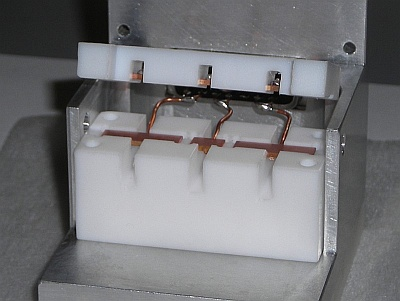
\includegraphics[width=0.6\textwidth]{figures/EOMinsidephoto.jpg}
\caption{Electro-optic modulator. \textcolor{blue}{Make a schematic
    drawing (crystal + electrodes + inductors) to accompany a picture
    like this one.}}
\label{fig:EOM}
\end{centering}
\end{figure}

\subsection{Mode cleaner}
The mode cleaner is a 12.2 m long suspended three mirror optical cavity
with finesse $\mathcal{F}=1282$ and free spectral range of
12.243~MHz. It is the first in-vacuum component the laser beam
encounters. The MC must transmit two of the sets of sideband light,
reject laser output that is not in the fundamental TEM$_{00}$ mode, and
play both a passive and active role in laser frequency stabilization
\cite{Zucker2002H1}.

\subsection{Faraday isolator}
The Faraday isolator is a three-port optical system that transmits
light straight through in one direction, yet rejects light traveling
in the opposite direction out of a third port. Crystals with a high
Verdet constant $\mathcal{V}$ and length $L$ sit in a magnetic field
with flux density $B$, rotating the polarization of the light passing
through by an angle $\beta = \int_0^L \mathcal{V} B(z) dz$, with $z$
the propagation direction. Polarizers outside of the magnetic field
purify the polarization of the light and send the backwards-traveling
rotated light out the third port, thus protecting the laser
source. This recovery of the reflected light from the interferometer
is also necessary for extracting length and angular information about
the interferometer's cavities. The Faraday isolator sits in the
interferometer vacuum system after the mode cleaner.

The Enhanced LIGO Faraday isolator design required more than simply
the use of low absorption optics. Even with minimal absorption, the
residual lensing and birefringence needed to be further mitigated
through additional design choices. Also, trade-offs between optical
throughput in the forward direction, optical isolation in the
backwards direction, and feasibility of physical access of the return
beam had to be considered. The result is that the Enhanced LIGO
Faraday isolator has a new layout and new optics compared to both the
Initial LIGO FI and typical commercial isolators.

Figure \ref{fig:FI} shows a schematic of the Enhanced LIGO Faraday
Isolator. It begins and ends with calcite wedge polarizers
(CWP). Between the CWPs is a thin film polarizer (TFP), a deuterated
potassium dihydrogen phosphate (DKDP) element, a half-wave plate
(HWP), and a Faraday rotator. The rotator is made of two low
absorption terbium gallium garnate (TGG) crystals and a quartz rotator (QR)
inside a 7-disc magnet with field strength of 1.16~T at its
maximum. The forward propagating beam upon passing through the
TGG, QR, TGG, HWP cascade is rotated by $+22.5^\circ -
67.5^\circ + 22.5^\circ - 22.5^\circ = 0^\circ$. In the backwards
direction, the rotation through HWP, TGG, QR, TGG is $-22.5^\circ +
22.5^\circ + 67.5^\circ + 22.5^\circ = 90^\circ$.

\begin{figure}
\begin{centering}
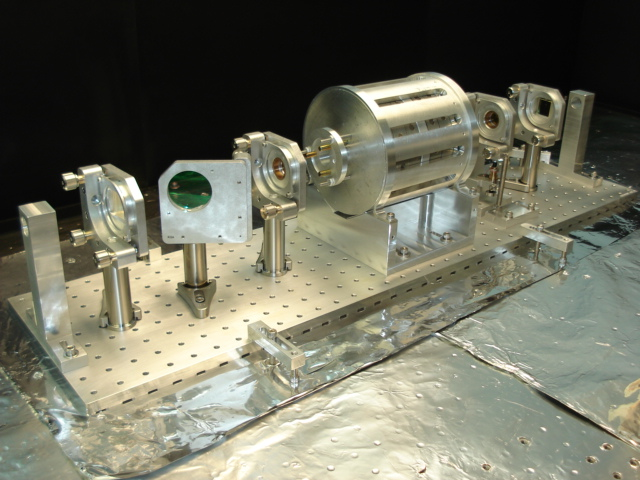
\includegraphics[width=0.6\textwidth]{figures/FI.jpg}
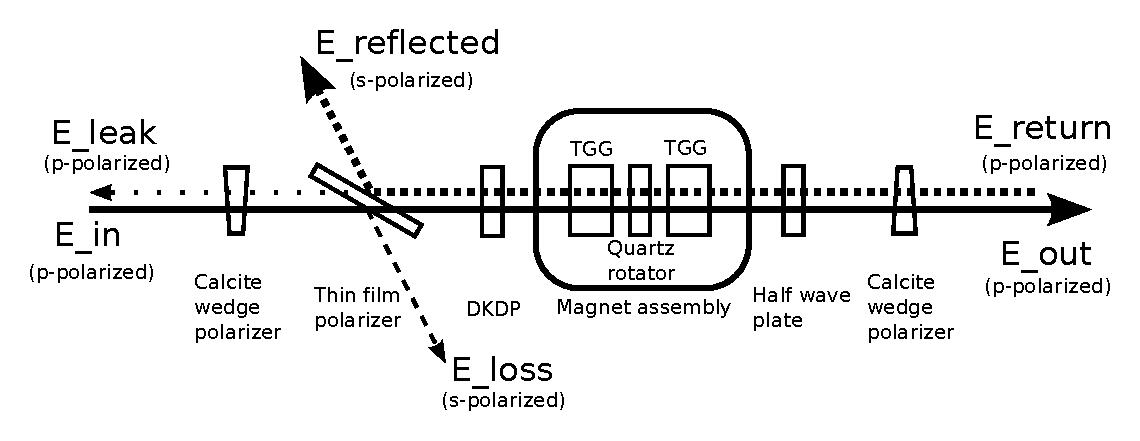
\includegraphics[width=1.0\textwidth]{figures/FaradayIsolator_nocolor.pdf}
%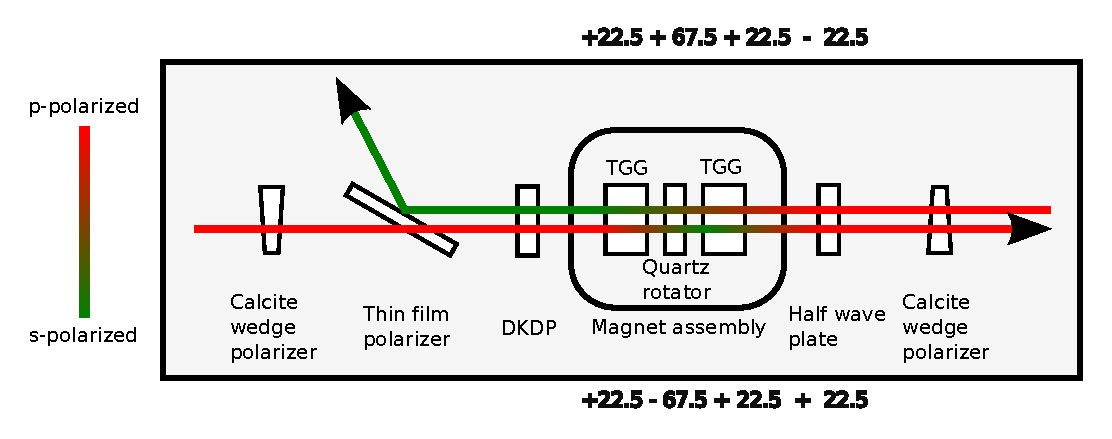
\includegraphics[width=1.0\textwidth]{/Users/kate/Documents/diagrams/FaradayIsolator.pdf}
\caption{Faraday isolator. The Faraday rotator preserves the light
  polarization in the forward-going direction and rotates it by 90
  degrees in the reverse direction. Fields are labeled for
  reference. \textcolor{blue}{Come up with better names. Overlay sketch of magnetic field
    strength? Show more realistic beam path angles?}}
\label{fig:FI}
\end{centering}
\end{figure}

\subsubsection{Thermal birefringence} 
Thermal birefringence is addressed by the use of two TGG crystals and
one quartz rotator rather than the typical single TGG. In this
configuration, any thermal polarization distortions that the beam
experiences while passing through the first TGG rotator will be
partially compensated upon passing through the second. The multiple
elements in the magnet requires a larger magnetic field than in Initial
LIGO and a Faraday
rotator housing that is 15.5~cm in diameter by 16.1~cm long.

\subsubsection{Thermal lensing}  
Thermal lensing is addressed by including DKDP, a negative $dn/dT$
material, in the beam path. Absorption of light in the DKDP results in
a de-focusing of the beam, which compensates for the thermal focusing
induced by absorption in the TGGs \cite{Khazanov2004Compensation}.

\subsubsection{Polarizers}  
The polarizers used (two CWPs and one TFP) each offer advantages and
disadvantages related to optical efficiency in one direction, optical
isolation in the other direction, and thermal beam drift. The CWPs
have very high extinction ratios ($>10^5$) and high transmission
(97\%), contributing to good optical efficiency and isolation
performance. However, the angle separating the exiting orthogonal
polarizations of light is very small, on the order of 10 mrad. This
requires relatively large distances to pick off the desired beams. In
addition, the 4.3$^{\circ}$ wedge angle of the CWPs enables thermal
drift. However, the CWPs as obtained from Karl Lambrecht for the
Enhanced LIGO Faraday are low absorption with expected total drift of
less than 100 $\mu$rad.

The advantages of the thin film polarizer over the calcite wedge
polarizer are that it exhibits negligible thermal drift at 30 W and it
is operates at the Brewster angle, thus diverting the return beam in
an easily accessible way. However, the TFP has a lower transmission
than the CWP and an extinction ratio of only 10$^3$. 

Thus, the combination of CWPs and a TFP combines the best of each to provide
a high extinction ratio (from the CWPs) and ease of reflected beam
extraction (from the TFP). The downsides that remain when using both
polarizers are that there is still some thermal drift from the
CWPs. Also the transmission is reduced due to the TFP and to the
fact that there are 16 surfaces from which light can scatter. 

\subsubsection{Heat conduction}
In an attempt to conduct some heat away from the Faraday components,
we wrapped the TGGs with indium foil that made contact with the
rotator housing. We also cushioned the DKDP and HWP with indium wire
in their holders.

\subsection{Mode matching telescope}
The mode matching telescope is a set of three suspended concave
mirrors that direct the light transmitted through the mode cleaner and
Faraday isolator to the interferometer. Located in the main vacuum
system, it must provide a beam whose mode characteristics match the
lowest order resonant mode of the interferometer arm cavities. The MMT
must also deliver the light to the interferometer without introducing
beam jitter.  Design considerations are discussed in
Ref. \cite{Delker1997Design}.



\section{Input Optics performance}
\label{sec:performance}
Perhaps the most convincing figure of merit for the Input Optics
performance is that the Enhanced LIGO interferometers achieved
low-noise operation with 20 W input power without excessive drift or
other annoyances. Additionally, the Input Optics were tested
successfully up to the available 30 W of power.  (Instabilities with
other interferometer subsystems limited the operation to 20 W.) We
present in this section details of the Input Optics performance during
Enhanced LIGO. Specific measurements and results discussed come from
Livingston; performance at Hanford was similar and is included in
tables summarizing the results.

\subsection{Optical efficiency}
The optical efficiency of the Enhanced LIGO Input Optics from EOM to
recycling mirror was 75\%, a marked improvement over the approximate
60\% of Initial LIGO. A substantial part of the improvement came
simply from the discovery and subsequent correction of a 6.5\% loss at
one of the in-vacuum steering mirrors directing light into the MC. A
45$^\circ$ reflecting mirror had been accidentally used for a beam
with an 8$^\circ$ angle of incidence. Losses attributable to the mode
cleaner and Faraday isolator are described below. A summary of the IO
power budget is found in Table \ref{tab:pwrbudget}.

\begin{table}
\centering
\begin{tabular}{l l l}
 & Livingston & Hanford \\
\hline\hline
Mode cleaner visibility & 92\% & 97\% \\
Mode cleaner transmission & 88\% & 90\% \\
Faraday transmission &       93\% & 94.4\%\\
\hspace{0.5cm} - Thin film polarizer loss &       4.0\% & 2.7\% \\ 
IO efficiency (PSL to RM) & 75\% & 82\% \\
\hline
\end{tabular}
\caption{Enhanced LIGO Input Optics power budget.}
\label{tab:pwrbudget}
\end{table}

\subsubsection{Mode cleaner losses} 
The mode cleaner was the greatest single source of power loss in both
Initial and Enhanced LIGO. The mode cleaner visibility, defined here as
\begin{equation}
\mbox{visibility} = (P_{input} - P_{reflected})/P_{input}, 
\end{equation}
the ratio of the amount of light coupled into the MC to the amount
sent at it, was 92\%. A result of higher order mode content and mode
mismatch into the MC, the visibility was constant up to 30~W input
power at both sites.

Then, of the light coupled into the mode cleaner, 88\% was
transmitted, corresponding to an average loss of 98 ppm per
mirror. Based on the mirrors' known surface micro-roughness, the
scatter loss is expected to be 22 ppm/mirror. Part of the discrepancy
between expectation and reality comes from poor AR coatings--we
measured a 1.3\% reflection off the should-be AR coating on MC mirrors
at both Livingston and Hanford, equivalent to a loss of 10~ppm per
mirror. In addition, a scan of the beam transmitted through the
mode cleaner gives $M^2$ values of less than 1 (see Fig. \ref{fig:MCtrans}), providing evidence for
clipping. In fact, MC2 has only a 1 inch clear aperture; minor
decentering can create losses. 

\begin{figure}
\begin{centering}
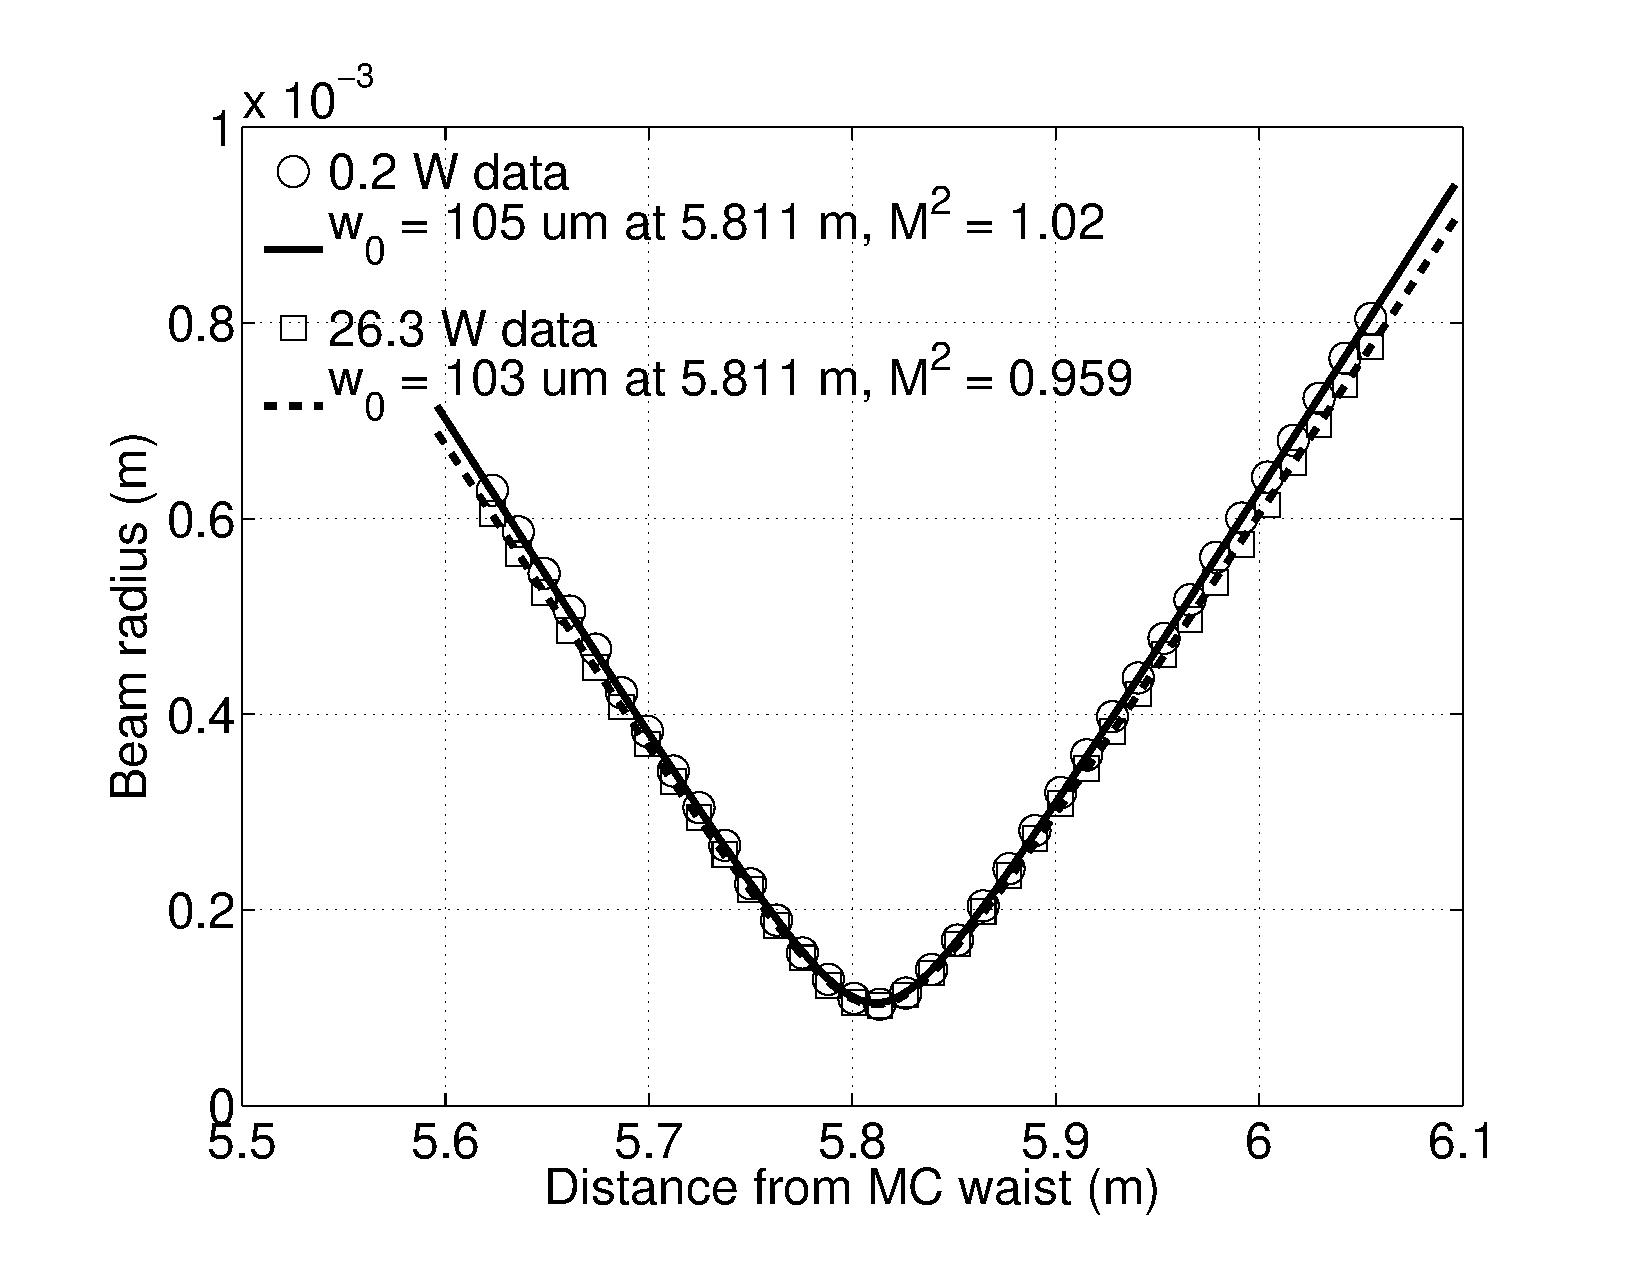
\includegraphics[width=0.7\textwidth]{figures/MCTrans_datafit.pdf}
\caption{Profile at high and low powers of a pick-off of the beam
  transmitted through the mode celaner.}
\label{fig:MCtrans}
\end{centering}
\end{figure}

Another source of MC losses is through absorption of heat by
particulates on the mirror's surface. Drag wiping the mirrors upon the
completion of Initial LIGO proved beneficial. The absorption decreased
from 18.7, 5.5 and 12.8 ppm per mirror, respectively, to 2.1, 2.0, and 3.4 ppm
per mirror. 

The measurement technique makes use of the thermally driven 28.2~kHz
drumhead eigenfrequencies (Fig. \ref{fig:MCpeaks}) of the mirror
substrate which serve as a monitor of the MC absorption via the
substrate's $dY/dT$. We cycled the power into the mode cleaner between
0.9~W and 5.1~W at 3 hour intervals, allowing for thermal
equilibrium. At the same time, we record the frequencies of the high Q
drumhead mode peaks as found in the mode cleaner frequency error
signal, heterodyned down by 28~kHz. Correcting for ambient temperature
fluctuations, we find a frequency shift of 0.043, 0.043, and 0.072
Hz/W. Refer to Tables \ref{tab:MCabsorption} and \ref{tab:MCabsorption2} and Figure
\ref{fig:MCabsorption}. A COMSOL model relates frequency shift to
absorption.

\begin{table}
\caption{Mode cleaner drumhead mode shift and absorption information.}
\centering
\begin{tabular}{l l l l}
mirror & frequency & frequency shift & absorption \\
\hline\hline
MC1 & 28.164 kHz & 0.043 Hz/W & 2.1 ppm \\
MC2 & 28.207 kHz & 0.043 Hz/W & 2.0 ppm \\
MC3 & 28.237 kHz & 0.072 Hz/W & 3.4 ppm \\
\hline
\end{tabular}
\label{tab:MCabsorption}
\end{table}

\begin{table}
\caption{Absorption values for the Livingston and Hanford mode
 cleaners before and after drag wiping. (For Hanford, association to
 a specific mode cleaner mirror is arbitrary.)}
\centering
\begin{tabular}{l l l l l}
 & Livingston & & Hanford & \\
mirror & before & after & before & after \\
\hline\hline
MC1 & 18.7 ppm & 2.1 ppm & 6.1 ppm & 5.8 ppm \\
MC2 & 5.5 ppm & 2.0 ppm & 23.9 ppm & 7.6 ppm \\
MC3 & 12.8 ppm & 3.4 ppm & 12.5 ppm & 15.6 ppm \\
\hline
\end{tabular}
\label{tab:MCabsorption2}
\end{table}


\begin{figure}
\begin{centering}
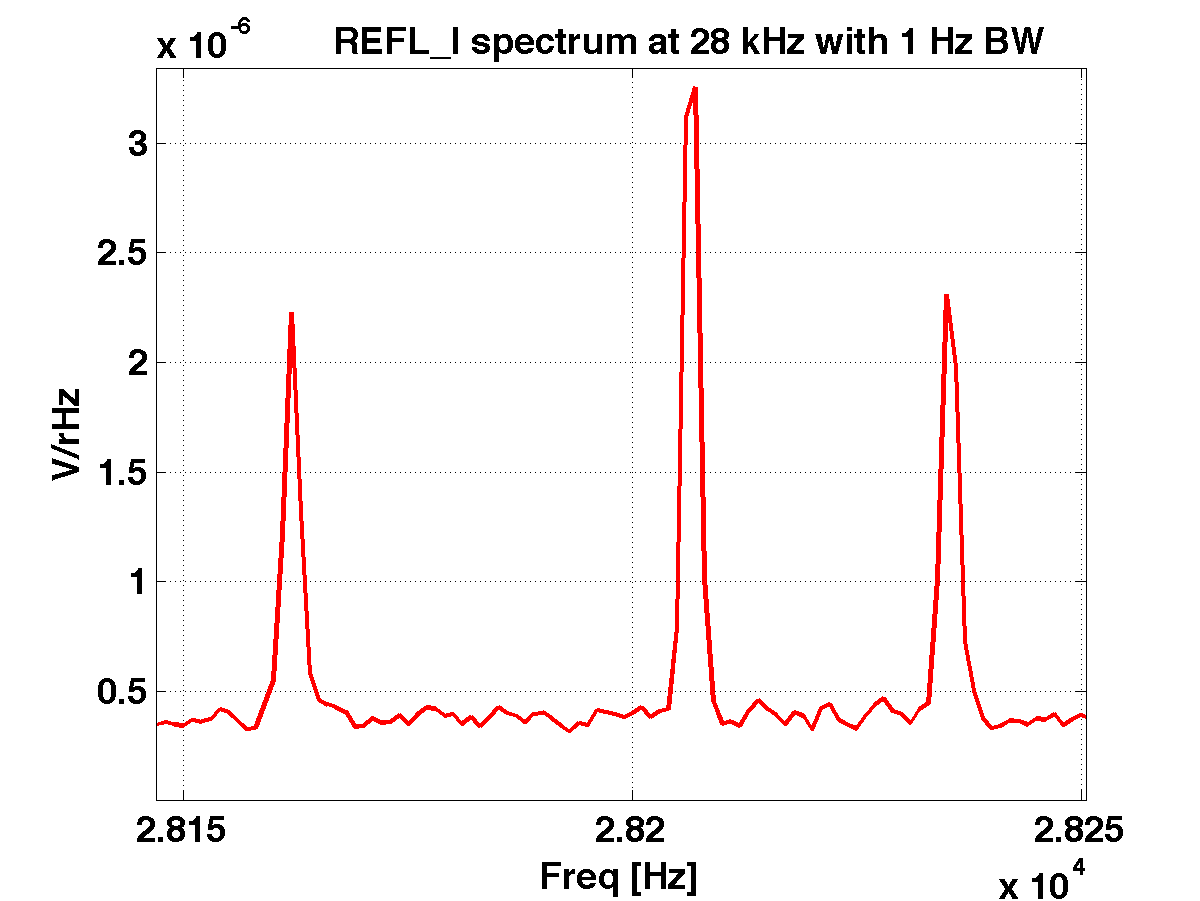
\includegraphics[width=1.0\textwidth]{figures/rana-1229241548.png}
\caption{MC drumhead mode peaks. \textcolor{blue}{This is Rana's plot; we don't have
  the original data. This is a png.}}
\label{fig:MCpeaks}
\end{centering}
\end{figure}


\begin{figure}
\begin{centering}
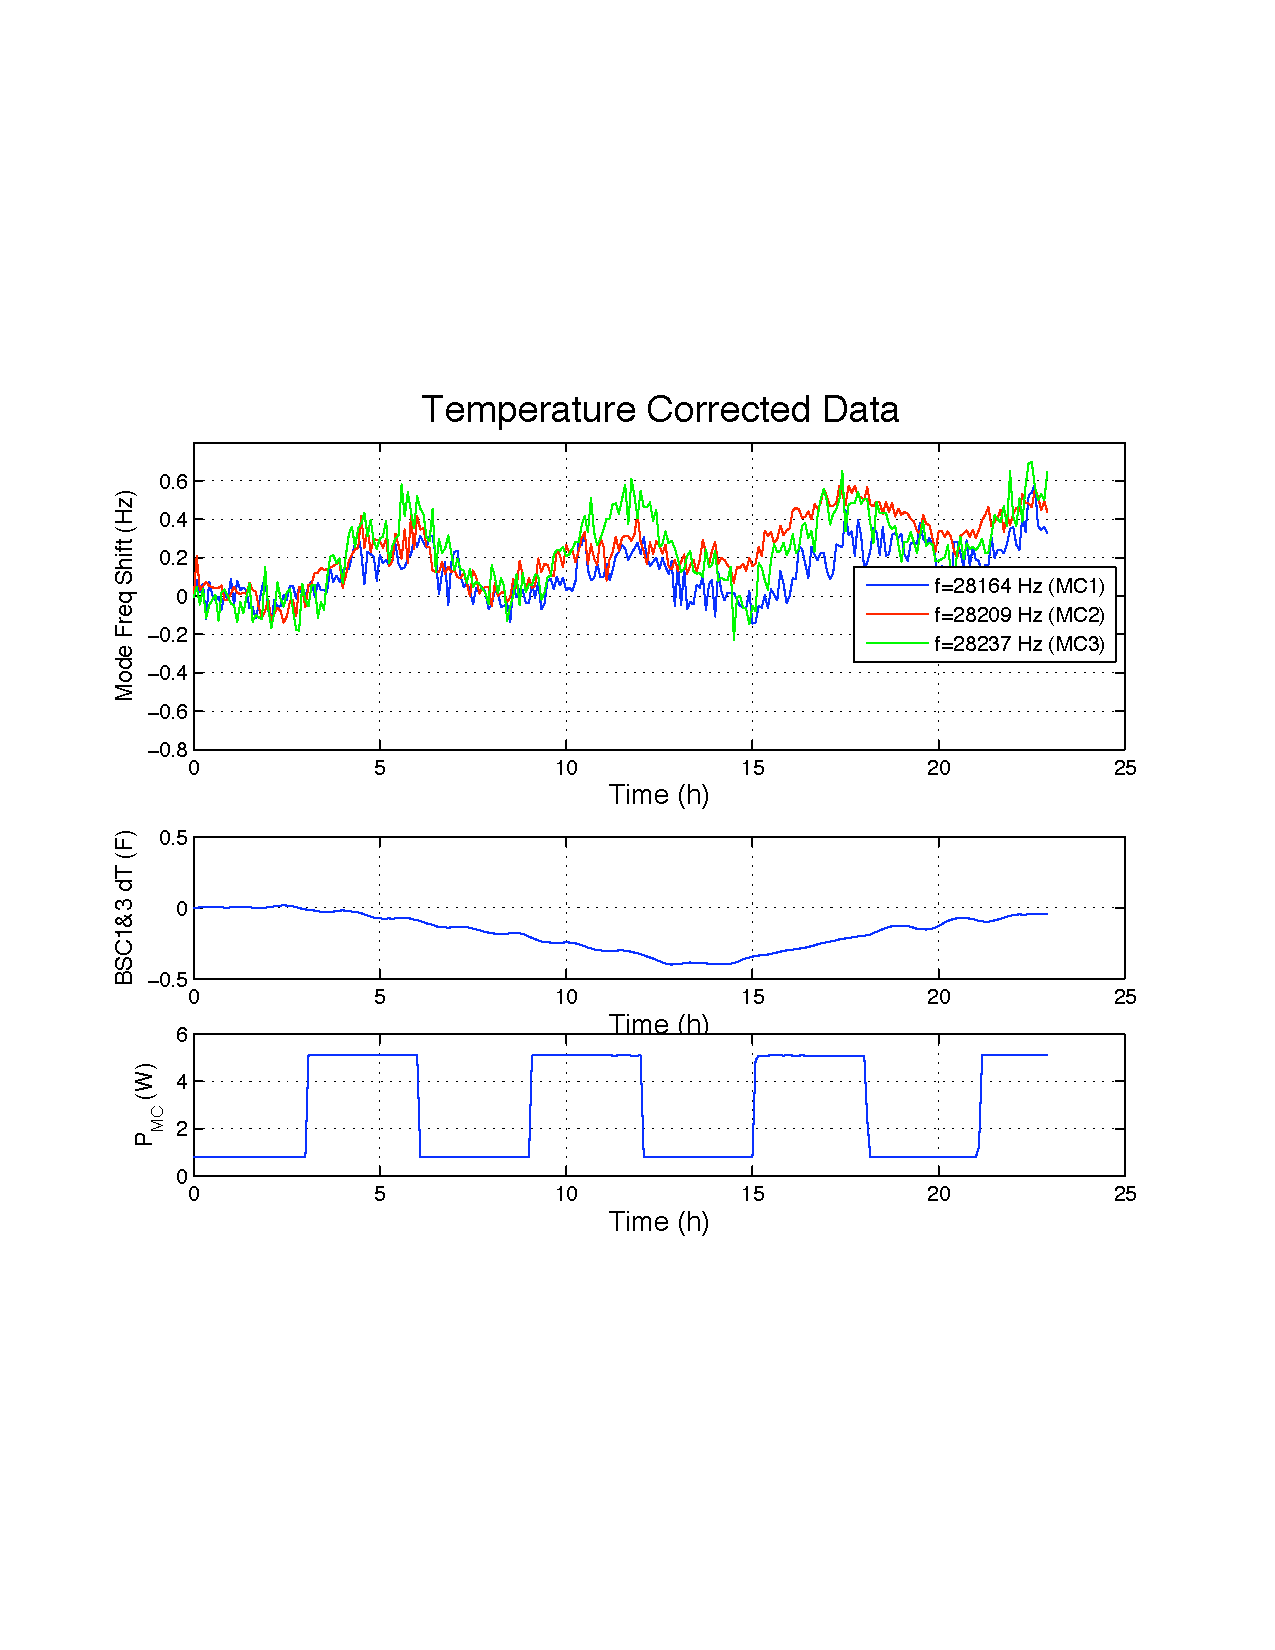
\includegraphics[width=1.0\textwidth]{figures/MCdrumheadFeb08_Tcorrected.pdf}
\caption{Mode cleaner absorption measurement. \textcolor{blue}{This is Valera's plot;
  we don't have original data. This is a pdf. This exact data set does
\emph{not} correspond to the data reported in Table
\ref{tab:MCabsorption}, but that table displays the cleanest analysis
we have.}}
\label{fig:MCabsorption}
\end{centering}
\end{figure}



\subsubsection{Faraday isolator losses} 
The Faraday isolator was the second greatest source of power loss with
a transmission of 93\%, better than the 86\% transmission
of the Initial LIGO FI. As expected, the lossiest element in the
Faraday isolator was the thin film polarizer, accounting for 4\% of
total losses. 



\subsection{Faraday isolation ratio}
The isolation ratio is defined as the ratio of power incident on the
Faraday in the backwards direction to the power transmitted in the
backwards direction:
\begin{equation}
\mbox{isolation ratio} = 10 \log_{10}(P_{in}/P_{out})
\end{equation}
We measured the isolation ratio of the Faraday isolator \emph{in situ}
through the use of two pick-offs of the backwards transmitted beam:
one was sent out of a vacuum chamber viewport immediately after
transmission through the Faraday and the other was picked off in air
further downstream just before entering the EOM in the backwards
direction. We misaligned the interferometer arms so that the input
beam would be promptly reflected off of the recycling mirror, thus
subjecting the Faraday rotator to twice the input power for this
measurement. As found in Figure \ref{fig:IR}, measurements at 1~W,
10~W, and 20~W input power show slight degradation of the Faraday's
isolation performance. We report a nominal in-vacuum isolation of 26
dB. For comparison, the isolation ratio
as measured in-air up to 25~W input power prior to installation was
34.4 dB.

\begin{figure}
\begin{centering}
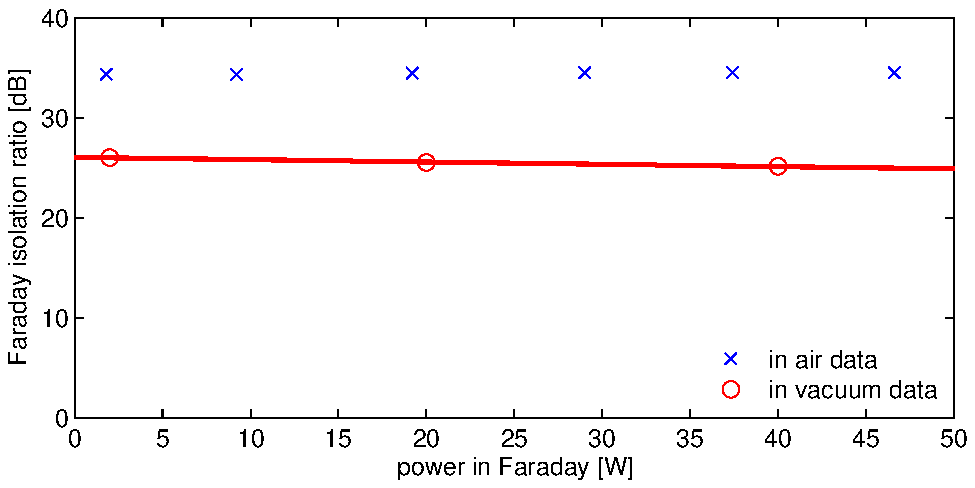
\includegraphics[width=0.7\textwidth]{figures/FaradayIR.pdf}
\caption{Faraday isolator isolation ratio as measured in air prior to
  installation and \emph{in situ} in vacuum.} 
\label{fig:IR}
\end{centering}
\end{figure}

\subsection{Thermal drift}
We measured the \emph{in situ} thermal drift of both the beam
transmitted through the mode cleaner and of the Faraday isolator up to
30~W input power. We misaligned the interferometer arms so that the
input beam would be promptly reflected off of the recycling mirror,
thus subjecting the Faraday rotator to 60~W total power for this
measurement.

As shown in Figure \ref{fig:drift}, the angle of the beam out of the
mode cleaner does not change as a function of power in yaw and changes
by 4.4$\times 10^{-7}$~rad/W in pitch. (\textcolor{blue}{pitch and yaw
  reversed?})  Tracking the backwards traveling beam rejected by the
Faraday isolator, we record a beam drift originating at the Faraday
rotator of 1.8$\times 10^{-6}$~rad/W in yaw and 3.2$\times
10^{-6}$~rad/W in pitch, also in Figure
\ref{fig:drift}. Therefore, when ramping the input power up to 30 W
during a full interferometer lock, the upper limit on the drift experienced by
the reflected beam is about 100 $\mu$rad. The active beam steering
system that had been required in Initial LIGO was no longer necessary
in Enhanced LIGO.
\begin{figure}
\begin{centering}
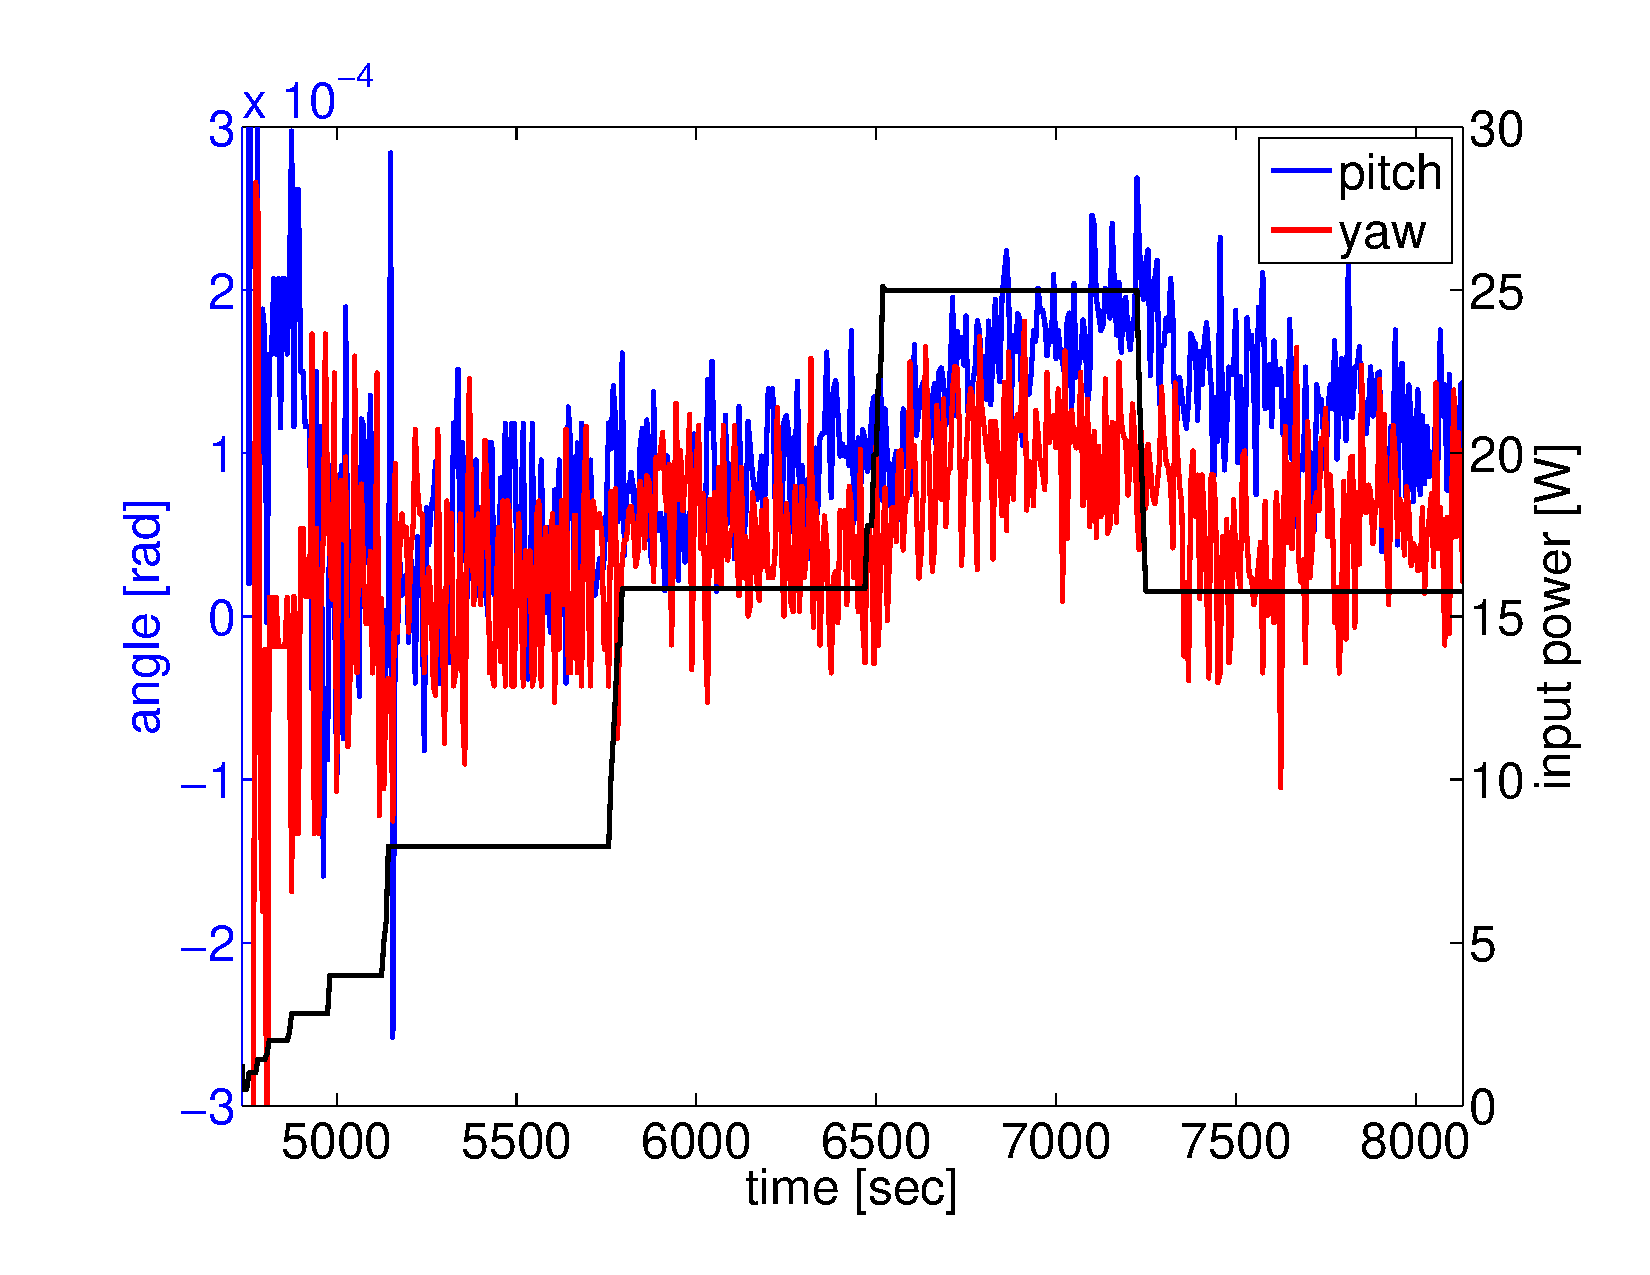
\includegraphics[width=0.7\textwidth]{figures/forpaper_refldrift.pdf}
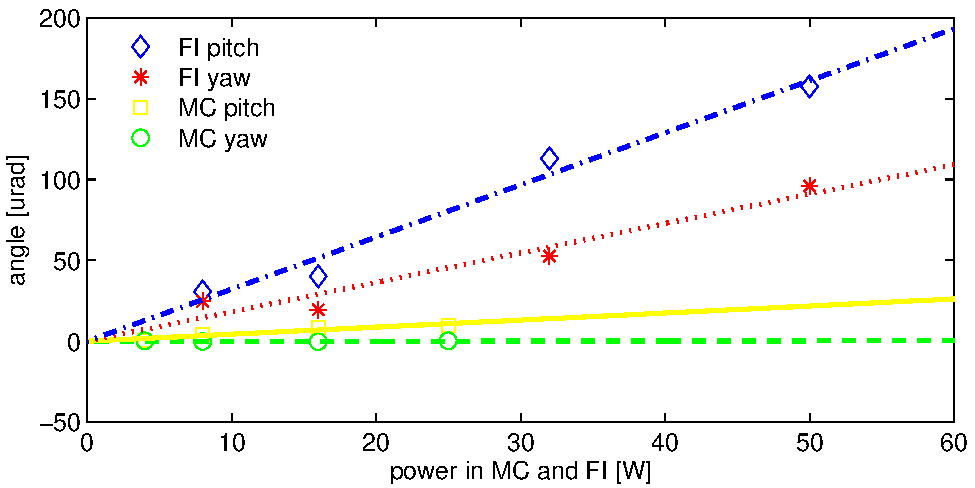
\includegraphics[width=0.7\textwidth]{figures/alldrift.pdf}
%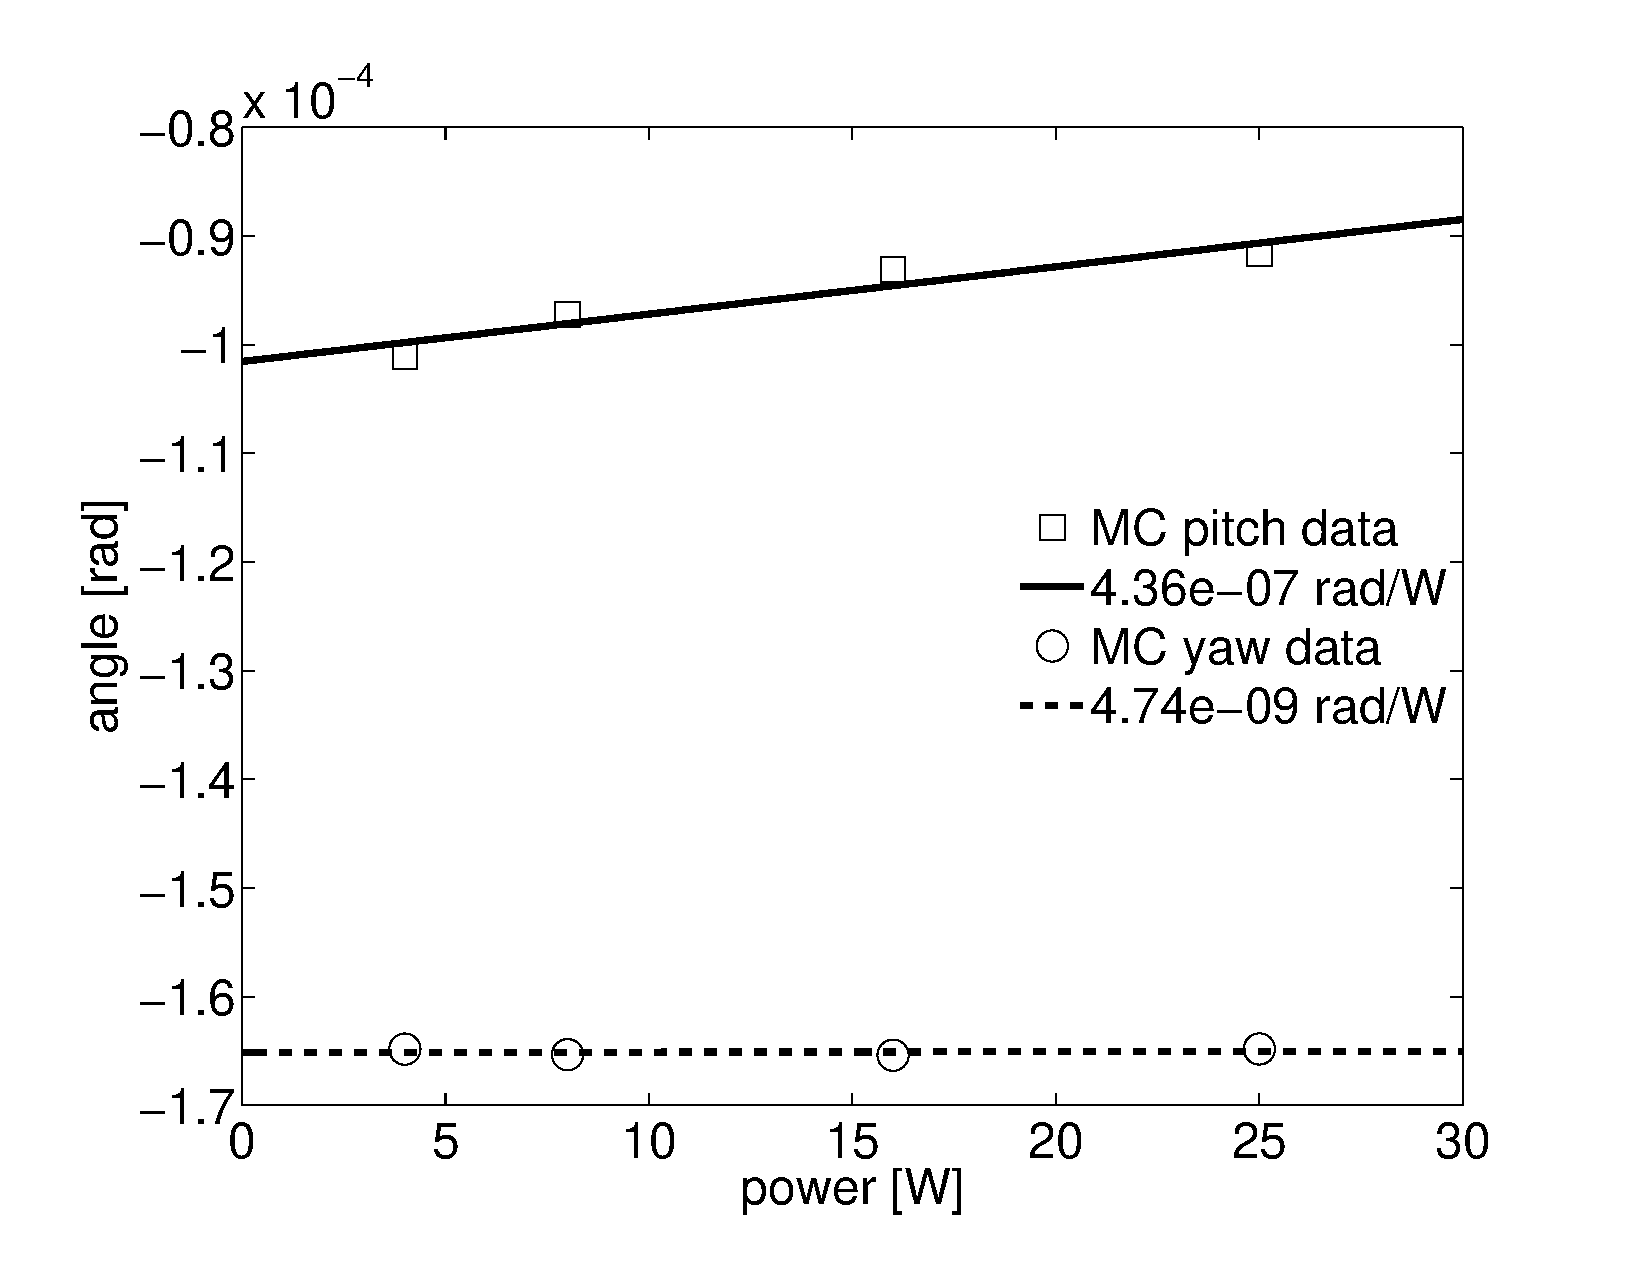
\includegraphics[width=0.7\textwidth]{/Users/kate/Documents/inputoptics/figures/MCdriftslopes.pdf}
\caption{Upper plot: FI drift data. Lower plot: Reduced mode cleaner and Faraday isolator thermal drift data. \textcolor{blue}{Since the beam travels twice through the Faraday isolator for
  this measurement, FI rad/W slopes should be divided by two.}}
\label{fig:drift}
\end{centering}
\end{figure}

\subsection{Thermal lensing}
Using a ThorLabs WM100 Omega Meter, we measured the profile of the beam rejected by the
Faraday isolator at low (1~W) and high (25~W) input power. As for the
thermal drift measurement, we misaligned the
interferometer arms so that the input beam would be promptly reflected
off of the recycling mirror. Picking off a fraction of the beam on the
in-air reflected port table, we measured the beam diameter at several
locations on either side of a beam waist. Refer to
Fig. \ref{fig:lensingsetup} for a diagram of our measurement
setup. A change in the beam waist size
or position from one power to the next would indicate the presence of
a thermal lens in the Faraday isolator. 

\begin{figure}
\begin{centering}

\includegraphics[width=0.7\textwidth]{figures/Setup_thermallensing.pdf}
%
\includegraphics[width=0.7\textwidth]{/Users/kate/Documents/diagrams/Setup_thermallensing.pdf}
\caption{Thermal lensing measurement setup.}
\label{fig:lensingsetup}
\end{centering}
\end{figure}

As seen in Fig. \ref{fig:lensing}, the waists of the two sets of data
are collocated--no thermal lens is measured. However, the divergence of
the beams differs, indicating that the beam quality degrades with
higher power. The $M^2$ factor at 1~W is 1.04 indicating the beam is
nearly perfectly a TEM$_{00}$ mode. At 25~W, $M^2$ increases to 1.19,
corresponding to increased higher order mode content. The percentage
of power in higher order modes depends strongly on the mode order and
relative phases of the modes, and thus cannot be determined from this
measurement \cite{Kwee2007Laser}.

\begin{figure}
\begin{centering}
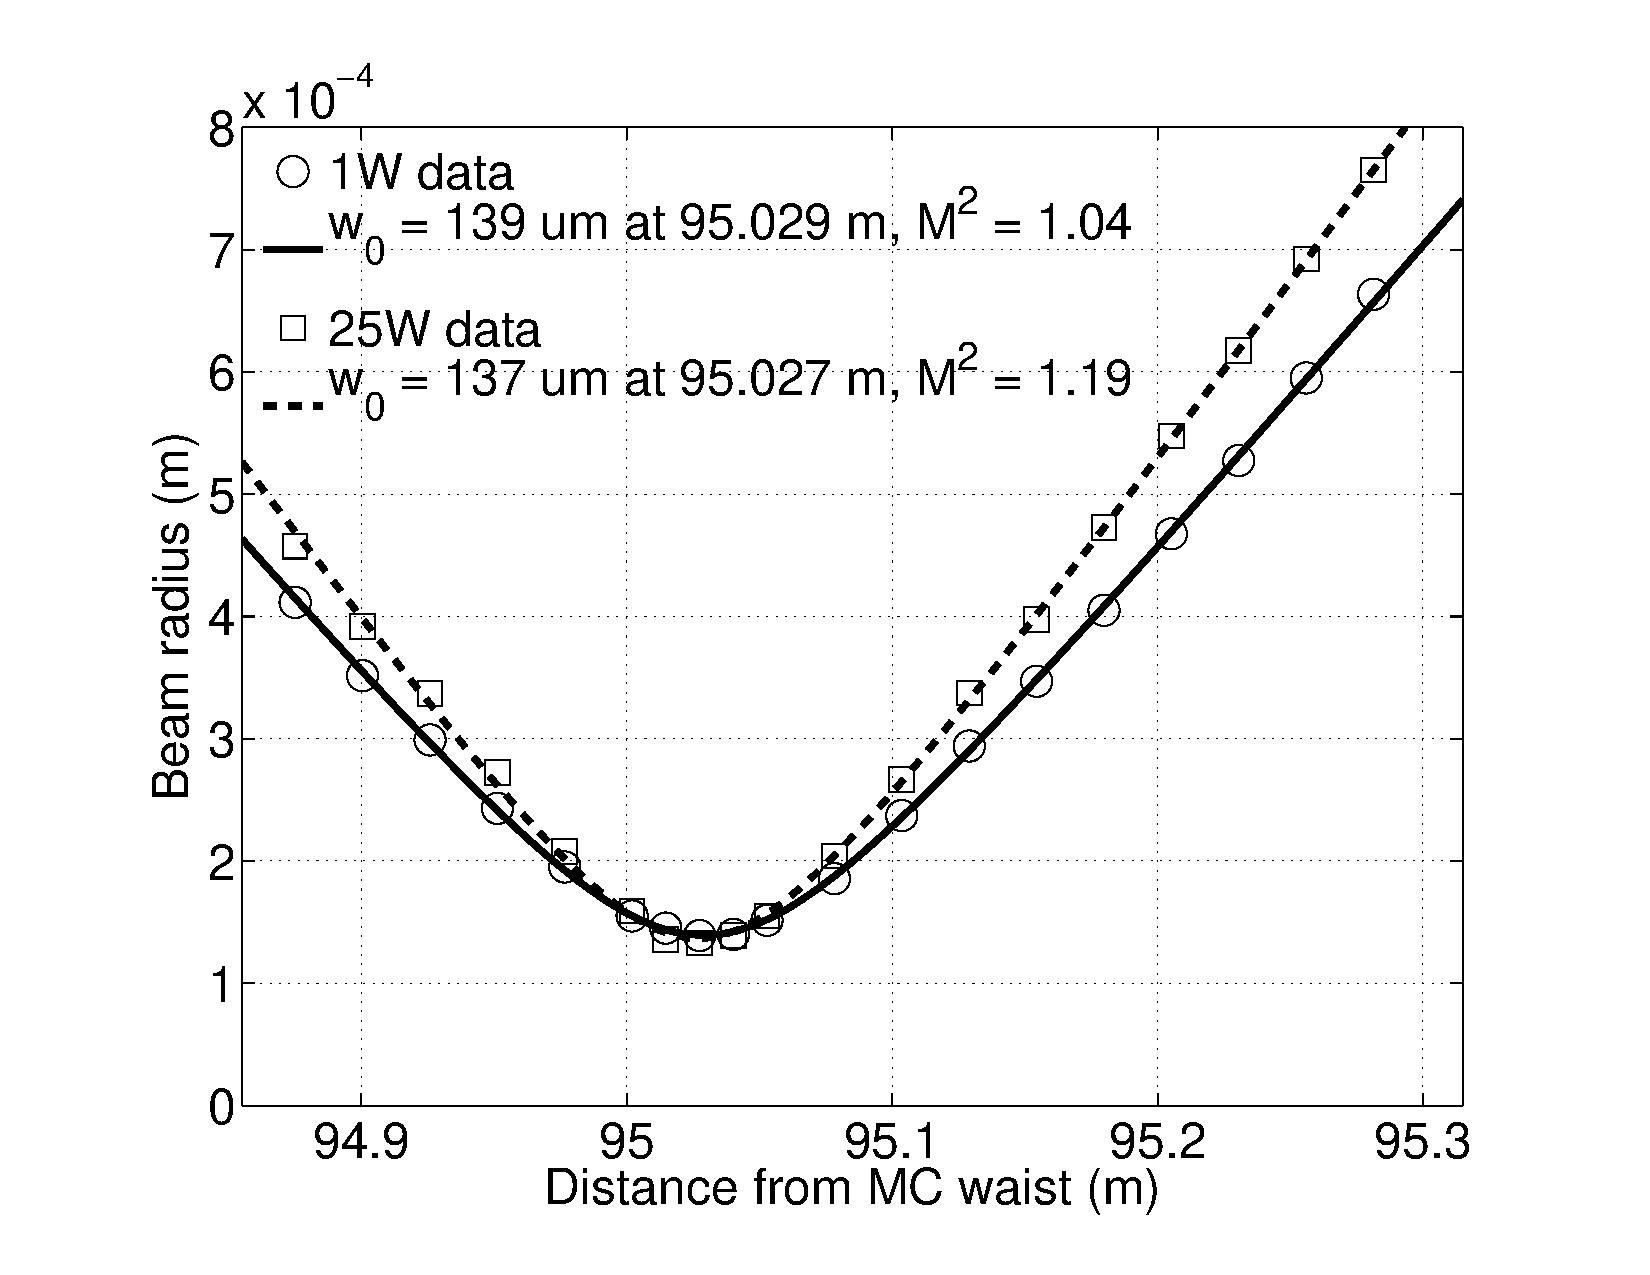
\includegraphics[width=0.7\textwidth]{figures/REFL_datafit.pdf}
%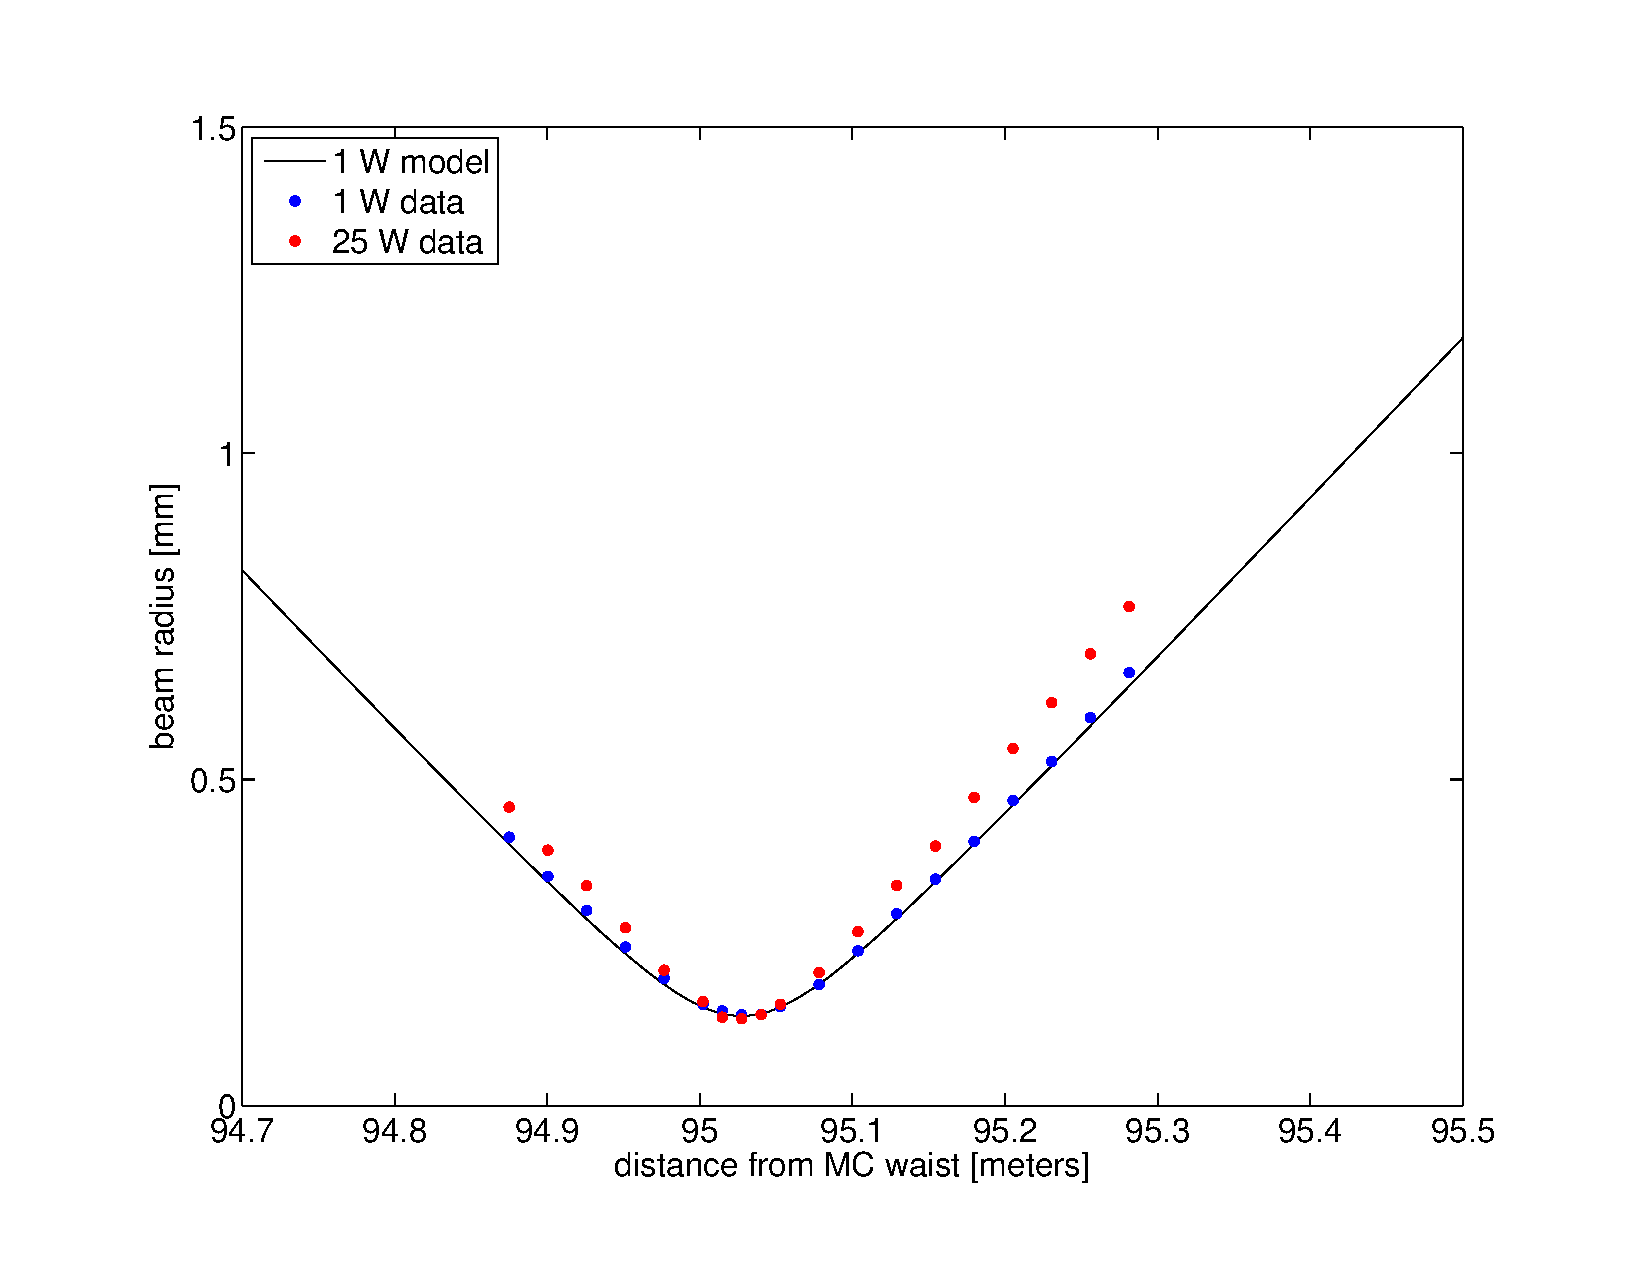
\includegraphics[width=0.7\textwidth]{/Users/kate/work/ioprofile/lensdata.pdf}
\caption{Faraday isolator thermal lensing data. With 25 W through the
  Faraday isolator one way, the beam has a steeper divergence than a
  pure TEM$_{00}$ beam, indicating the presence of higher order modes.}
\label{fig:lensing}
\end{centering}
\end{figure}

\subsection{Mode matching}
We can measure the effectiveness of the mode-matching telescope by
taking the ratio of power at the reflected port when all of the
interferometer cavities are on resonance to the power in the reflected
beam when the cavities are unlocked. Since the impedance matching is near perfect,
all light at the reflected port during interferometer lock is
attributable to a mode mismatch. The ratio we measure is 8\%, meaning
the MMT succeeds at coupling 92\% of the light into the
interferometer. 

\subsection{EOM}
\textcolor{blue}{What to say here?}




\section{Discussion}
\label{sec:aLIGO}
We demonstrate that the Enhanced LIGO Input Optics enable the
possibility of high power interferometry without adverse side
effects. Table \ref{tab:summary} summarizes the IO performance in
Enhanced LIGO for both Livingston and Hanford.
\begin{table}
\caption{Enhanced LIGO Input Optics performance summary.}
\centering
\begin{tabular}{l l l}
 & Livingston & Hanford \\
\hline\hline
IO transmission & 75\% & 82\% \\
Faraday Isolation & 26 dB & \\
Faraday thermal drift & 3 $\mu$rad/W & not measured \\
IO thermal lensing & negligible & not measured \\
Mode matching & 92\% & \\
\textcolor{blue}{Something else} & & \\
\hline
\end{tabular}
\label{tab:summary}
\end{table}

An important function of Enhanced LIGO was the demonstration of
prototype Advanced LIGO technologies. The Enhanced LIGO Input Optics
served just that purpose. Although they were subjected to at most only
20~W of input power on a regular basis, the improved performance
over the Initial LIGO IO operating at 7~W input power proves the
success of their design. 

The Input Optics still, however, needs to work just as well with 10
times more power for Advanced LIGO. Neither the mode cleaner nor EOM
showed any degradation, so projections to Advanced LIGO cannot be
made. (\textcolor{blue}{mode cleaner radiation pressure effects?})
Mode matching was constant with power, as was mode cleaner visibility
and the Faraday isolation ratio. Given a Faraday isolator thermal
drift of 3 $\mu$rad/W, we can expect 600 $\mu$rad/W
drift in Advanced LIGO. More higher order mode content will also be
generated.